\documentclass[12pt,a4paper,onecolumn]{article}

%%%%%%%%%%%%%%%%%%%%%%%%%%%%%%%%%%%
%          				PACKAGES  				              %
%%%%%%%%%%%%%%%%%%%%%%%%%%%%%%%%%%%

%\usepackage[margin=1in]{geometry}
\usepackage[top=2cm, bottom=2cm, left=2cm, right=2cm]{geometry}

\usepackage{authblk}
\usepackage{amsfonts}
\usepackage{graphicx,color}
\usepackage{amsmath}
\usepackage{amssymb}
\usepackage[table]{xcolor}
\usepackage{setspace}
\usepackage{booktabs}
\usepackage{dcolumn}
\usepackage{rotating}
\usepackage{color,soul}
\usepackage{threeparttable}
\usepackage[capposition=top]{floatrow}
\usepackage[labelsep=period]{caption}

\usepackage{subcaption}
\usepackage{lscape}
\usepackage{pdflscape}
\usepackage{multicol}
\usepackage[bottom]{footmisc}
\setlength\footnotemargin{5pt}
\usepackage{longtable} %for long tables

\usepackage{enumerate}
\usepackage{units}  %nicefraction
\usepackage{placeins}
\usepackage{booktabs,multirow}
%% BibTeX settings
\usepackage{natbib}
\bibliographystyle{apalike}
%\bibliographystyle{unsrtnat}
\bibpunct{(}{)}{,}{a}{,}{,}

% Codificación y tipografías correctas
\usepackage[utf8]{inputenc}   % permite escribir áéíóúñ directamente
\usepackage[T1]{fontenc}      % hyphenation y copiado correcto con 
\usepackage{lmodern}          % fuentes con T1 (Latin Modern)

\usepackage{enumitem} % listas sin sangría extra

%% paragraph formatting
\renewcommand{\baselinestretch}{1}


% Defines columns for tables
\usepackage{array}
\newcolumntype{L}[1]{>{\raggedright\let\newline\\\arraybackslash\hspace{0pt}}m{#1}}
\newcolumntype{C}[1]{>{\centering\let\newline\\\arraybackslash\hspace{0pt}}m{#1}}
\newcolumntype{R}[1]{>{\raggedleft\let\newline\\\arraybackslash\hspace{0pt}}m{#1}}



\usepackage{comment} %to comment entire sections

\usepackage{xfrac} %sideways fractions


\usepackage{bbold} %for indicators

\setcounter{secnumdepth}{6}  %To get paragraphs referenced 

\usepackage{titlesec} %subsection smaller
\titleformat*{\subsection}{\normalsize \bfseries} %subsection smaller
%\usepackage[raggedright]{titlesec} % for sections does not hyphen words


\usepackage[colorlinks=true,linkcolor=black,urlcolor=blue,citecolor=blue]{hyperref}  %Load last
%% markup commands for code/software
\let\code=\texttt
\let\pkg=\textbf
\let\proglang=\textsf
\newcommand{\file}[1]{`\code{#1}'}
\newcommand{\email}[1]{\href{mailto:#1}{\normalfont\texttt{#1}}}
\urlstyle{same}
%%%

\usepackage{makecell}

\usepackage{graphicx}

% Tables and safe variable names (ASCII only)
\usepackage{longtable,booktabs,array,ragged2e,seqsplit}
\newcolumntype{L}[1]{>{\RaggedRight\arraybackslash}p{#1}}
\newcommand{\var}[1]{\texttt{\seqsplit{\detokenize{#1}}}} % breakable, no need to escape _

\usepackage[colorlinks=true,linkcolor=black,urlcolor=blue,citecolor=blue]{hyperref}



%%%%%%%%%%%%%%%%%%%%%%%%%%%%%%%%%%%
%     			TITLE, AUTHORS AND DATE    			  %
%%%%%%%%%%%%%%%%%%%%%%%%%%%%%%%%%%%

\title{\textbf{Of Reason, Faith, and Models: An Efficient Machine Learning Approach to Predicting Poverty in Colombia}}

%\large {Machine Learning and Big Data, School of Economics, Universidad de los Andes}

\author{Juan Jos\'e Rojas, Francisco Soler, Jes\'us Yancy }

\date{}

%%%%%%%%%%%%%%%%%%%%%%%%%%%%%%%%%%%
%          				  DOCUMENT       					      %
%%%%%%%%%%%%%%%%%%%%%%%%%%%%%%%%%%%

\begin{document}
\maketitle
\thispagestyle{empty}
\begin{center}
\texttt{Link to the GitHub repository: \url{https://github.com/jrconstain/PS2_Group4}}
\end{center}


\section{Introduction}

In 2024, 16.2 million Colombians—31.8\% of the population—lived in households with a per capita income below the national poverty line. This line is constructed estimating the cost of minimum caloric intake (the extreme poverty line) and then scaling it using the Orshansky coefficient\footnote{ \emph{Orshansky coefficient} is the multiplier used to convert a food-only
poverty line into a total (food + non-food) poverty line:
\( \mathrm{LP} = \mathrm{LPE} \times \mathrm{Orshansky} \), where
\( \mathrm{Orshansky} = \frac{\text{total household expenditure}}{\text{food expenditure}} \)
for a designated reference group and estimated empirically by geography \citep{DANE2025a}.}, estimated for each geographic domain from empirical household spending patterns \citep{DANE2025a}. For 2024, this translated into monthly per capita thresholds of COP 227,22 and COP 460,198 \citep{DANE2025b}. Falling below that line could not exactly mean hunger, but it means being unable to participate fully in economic life. It implies not having enough money to afford clothes, transportation, basic repairs, or recreation. It means lacking any margin for emergencies, improvement, or to invest in one’s future. Poverty is then both a personal tragedy and a collective inefficiency: it denies individuals a dignified life and prevents millions from taking part in the very markets that sustain collective prosperity.

That’s why reducing poverty remains one of the central goals of scientists, governments and global institutions. But identifying what works, requires first being able to measure poverty accurately, which in turn imply collecting detailed household surveys that are time-consuming, costly, and logistically demanding. If we could estimate poverty reliably using fewer questions, meaning cheaper surveys, we might be able to expand coverage, monitor policies more effectively, and ultimately improve the lives of millions \citep{DrivenData2018Poverty}. This is where Machine Learning can help. As a statistical-computational tool suitable for prediction, it could allow us to uncover patterns in existing data that help design more efficient poverty measurements. 

In this Problem Set, we address this challenge by applying ML techniques to predict poverty in Colombia using data from the 2018 \emph{Gran Encuesta Integrada de Hogares} (GEIH)\citep{DANE2025c}. The dataset comprises 164,960 observations at the household level for model training and an additional 66,168 for out-of-sample evaluation in a \href{https://www.kaggle.com/competitions/uniandes-bdml-2025-20-ps-2/overview}{Kaggle competition} organized as part of the Big Data and Machine Learning 2025-2 course at Universidad de Los Andes. The GEIH provides detailed labor, economic, and demographic information at both the individual and household levels, including employment status, income sources, education, and housing conditions. We aimed to build an accurate predictive model and identify the most informative signals that can make poverty measurement faster, cheaper, and more actionable for public policy.

In the breakthrough paper of Google Flu Trends, authors reportedly estimated a total of \char`~450 million models to predict influenza outbreaks--an illustration of the vast decision space that machine learning entails \citep{Google2009}. To tackle efficiently our prediction problem, we decided to frame this space along three dimensions, each requiring a distinct approach: variables, models, and hyperparameters. Variables call for deep undestanding of problem’s fundamentals and domain knowledge to identify and construct features that meaningfully relate to the phenomenon under study. Models, in turn, require technical expertise in machine learning to identify which algorithms are best suited to capture the relationships between variables--i.e. that could most closely represets the real $f(x)$--, and to apply each method with sound reasoning. Finally, hyperparameters invite systematic exploration: grid searches with cross-validation serve as controlled experiments (or structured brute-force approaches) that test combinations across a defined range of possibilities to uncover the most efficient configurations.

Although we understand that machine learning is not deterministic, and that alternative combinations of features or methods might yield better results in the abstract space of possibilities, we adopted an experimental mindset throughout the process, allowing us to advance iteratively and with purpose. By changing one element at a time and holding others constant, we could causally attribute prediction improvements to specific decisions. Our approach was, in a sense, a Kierkegaardian act of faith, but one grounded in the reasoning that thoughtful modeling and deep problem understanding increase the odds of finding the right path, far more than random exploration. 

This strategy proved effective. We began by establishing a baseline using simple logistic regression models and iteratively expanding the feature set to over 20 variables, which allowed us to achieve an out-of-sample F1 score of 0.62. Introducing regularization with Elastic Net, along with hyperparameter tuning and threshold optimization, brought us to 0.65. While CART underperformed with an F1 of 0.48, we advanced toward more sophisticated tree-based methods--Random Forest and Gradient Boosting-- which, applied to the same feature set with corrected imputation, increased our score to 0.70. Building on that, we carefully designed our final set of features through deep, problem-driven analysis, pushig our best Gradient Boosting model to a 0.72 score. Finally, an XGBoost model, trained on the complete engineered feature set with full optimization applied, achieved an out-of-sample F1 of 0.74 on 20\% of the test data. This placed us at the top of the \href{https://www.kaggle.com/competitions/uniandes-bdml-2025-20-ps-2/leaderboard}{Kaggle
 competition leaderboard} (temporarily, pending final evaluation), doing so with less than half the submission attempts than the next best team.\footnote{Remarkably, computations for this best model were performed on a standard consumer laptop (8 GB RAM, 4 CPU cores), underscoring the efficiency and accessibility of our approach.}


%%% Intructions: The introduction states the problem and any antecedents. It briefly describes the data and its suitability to address the problem set question. It contains a preview of the results and main takeaways. Keep this section up to 5 paragraphs.

\section{Data}

For this Problem Set, we were given a subset of the 2018 \textit{Gran Encuesta Integrada de Hogares} (GEIH), a nationally representative household survey conducted by DANE. The dataset includes variables on employment status, income sources, education, housing conditions, and household composition. The training data comprise 543,109 individual observations and their corresponding 164,960 households, while the test data include 219,644 individuals into 66,168 households.  In the training data, household income is observed; however, in the test data it is not provided as it would allow for a deterministic calculation of monetary poverty. Moreover, this omission reflects the difficulty and cost of measuring income directly.

In machine learning, as in many areas of science and engineering, half of the solution almost always lies in defining the problem clearly. In our case, the target variable is deterministically defined as
$Poor = I(Income_{p.c.} < L_p)$, where \(L_p\) denotes the poverty line established by DANE for an specific area. Since \(L_p\) is known, its information can be incorporated into the model, effectively transforming the task into predicting whether the household’s total income, divided among its members, is sufficient to surpass this line. This denominator is the number of household members sharing total expenditures (\(N_{\text{persug}}\)), that we also included as a structural predictor. Moreover, the total income variable used for the calculation includes imputed rent (\textit{arriendo imputado}), making variables describing housing tenure an essential feature to include.

From this point onward, we leveraged our domain knowledge as economists to focus on identifying and constructing variables that could contain strong signals of household income. The first problem set of the course was especially valuable in this regard, as it highlighted the predictive power of variables such as education, sex, and age for individual income. This experience guided us in thinking more systematically about how household composition, labor status, and human capital characteristics interact to determine overall income levels.

% === Macro SIN paquetes para mean con SE debajo ===
\newcommand{\meanse}[2]{%
  \begin{tabular}{@{}c@{}}%
    #1\\[-0.1ex]\footnotesize(#2)%
  \end{tabular}%
}

% --- Compacidad / ancho ---
\setlength{\tabcolsep}{2.5pt}  % más angosta que el default
\renewcommand{\arraystretch}{1.03}

\begin{table}[!htbp]\centering
\footnotesize
{\footnotesize
  \caption{Train Sample (Houshold level) — Panel A: Numeric variables and Panel B: Categorical variables by poverty status}
  \label{tab:table1}
  % p{...} angosta la primera columna; @{} elimina márgenes laterales
  \begin{tabular}{@{}p{0.44\linewidth}cc@{}}
    \hline
    \multicolumn{1}{l}{\textit{Households (N)}} & \multicolumn{2}{c}{\textit{164,960}} \\
    \hline
    \multicolumn{3}{l}{\textbf{Panel A. Numeric variables — mean (SE)}} \\
    Variable
      & \begin{tabular}{@{}c@{}}\textbf{Poor}\\[-0.2ex]\footnotesize(N = 33,024)\end{tabular}
      & \begin{tabular}{@{}c@{}}\textbf{Non-poor}\\[-0.2ex]\footnotesize(N = 131,936)\end{tabular} \\
    \hline
    Number of people in the household’s expenditure unit. & \meanse{4.131}{0.011} & \meanse{3.066}{0.005} \\
    Imputed/estimated rent & \meanse{132777.053}{12425.517} & \meanse{347537.237}{9533.729} \\
    Rent payment (actual rent paid) & \meanse{138667.384}{1143.817} & \meanse{179218.542}{2847.215} \\
    Age of the head of household & \meanse{46.773}{0.089} & \meanse{50.323}{0.045} \\
    Hours worked by the head of household & \meanse{28.620}{0.139} & \meanse{34.493}{0.068} \\
    Number of employed persons in the household & \meanse{1.257}{0.005} & \meanse{1.566}{0.003} \\
    Number of unemployed persons in the household & \meanse{0.319}{0.003} & \meanse{0.148}{0.001} \\
    Average hours worked among employed persons & \meanse{34.366}{0.120} & \meanse{40.348}{0.052} \\
    Proportion of employed persons relative to the number of people in the household & \meanse{0.311}{0.001} & \meanse{0.545}{0.001} \\
    \hline
    \multicolumn{3}{l}{\textbf{Panel B. Categorical variables — mode}} \\
    \hline
    Home ownership status & Rented or sublet & Owned, fully paid \\
    Sex of the head of household & Male & Male \\
    Contributes to pension (head) & No & No \\
    Occupational position of the head of household & Self-employed & Self-employed \\
    Highest education level of the head of household & Primary & University. \\
    \hline
  \end{tabular}
} % fin \footnotesize
\end{table}





First, to better capture individual educational attainment, we derived \textit{years of education} from two GEIH questions (\texttt{p6210} and \texttt{p6210s1}), by summing the years required to get to the highest level attained and years reported as completed within that level. From there, we aggregated a wide range of individual-level features to build household-level indicators that reflected demographic structure and productive capacity. Examples include the average years of education among employed members, the proportion of employed individuals relative to household size, and the average number of hours worked by these members. We also incorporated characteristics of the household head—such as age, sex, education, pension contributions, tenure, and firm size—alongside composite indicators like whether any employed member received formal benefits. Together, these variables aim to capture dimensions of job quality and informality that are central to understanding poverty status. In addition, we constructed variables based on the sources of income. For example, one indicator captured whether any household member received income from capital sources--rents, dividends, or interest payments--a variable that proved particularly informative in some of our models. A complete dictionary of all variables used and created for our models is available in \hyperref[tab:vars]{Table~A1} of the Appendix. 

To address missing values in the data, we applied targeted imputation strategies based on the nature of each variable. These included median or mode imputation, assigning NA = 0 when appropriate, and replacing missing entries with predefined labels established by the survey design.

\hyperref[tab:table1]{Table~1} summarizes key household-level differences by poverty status in our consolidated dataset. The first thing to note is the strong class imbalance, with 80\% of our sample is classified as \textit{No Pobre}, which will later require attention through corrective strategies to avoid biased model performance. Moreover, a clear pattern emerges: although poor and non-poor households share similar modes in job type (\textit{cuenta propia}) and pension status (\textit{no}), they differ sharply in intensive margins like total hours worked. This aligns with Banerjee and Duflo’s (2011) “ladders and snakes” view, where small labor market frictions compound into large income gaps. Notably, the employed-to-household-size ratio shows substantial disparity, being
0.31 among the poor versus 0.54 among the non-poor. For its part, panel B highlights that poor households are more likely to rent and pay lower rents, reflecting thinner asset buffers and reduced access to credit and opportunity. 

These are precisely the kind of signals a prediction-first approach can exploit. Our feature engineering thus focused on ratios, head characteristics, and tenure, capturing structural constraints in compact, survey-friendly variables. Building on this, we expanded the feature set with nonlinear transformations and interactions to enable models to learn complex complementarities.
 

\section{Models and Results}

\subsection{Classification Models}
Our modeling strategy was guided by an experimental, incremental approach: we varied one element at a time--whether features, model type, or hyperparameters--and tracked its impact on out-of-sample performance. This allowed us to iteratively refine our pipeline based on measurable improvements. This section will continue this same strategy by explaining -step by step- the decision taken to achieve the highest scoring model in our objective to predict \textit{pobre} (pobre=1) and \textit{no pobre} (pobre=0). Table 2 summarizes the models we tested, their corresponding feature sets, and out-of-sample F1 scores.
\begin{table}[h!]
\footnotesize
\caption{Model's out-of-sample F1 score and Dataset Specifications} 
\centering
\begin{tabular}{l c c c c c c c}
\hline
\textbf{Model} & \textbf{Score} & $\varnothing$ & (1) & (2) & (3) & (4)  \\
\hline
Logit 1 & 0.36 & X &   &   &   &     \\
Logit 2 & 0.57 &   & X &   &   &     \\
Logit 3 & 0.62 &   &   & X &   &     \\
Elastic Net  1    & 0.60 &   &   &  X &  &     \\
CART 1   & 0.48 &   &  & X  &   &     \\
Random Forest 1    & 0.65 &   &  &  X &   &     \\
Random Forest 2 (TH OP) & 0.68 &   &   & X &   &   \\
Random Forest 3 (TH OP) & 0.69 &   &   &   & X &   \\
Gradient Boosting 1    & 0.70 &   &   &   & X &    \\
Random Forest 4 (TH OP) & 0.71 &   &   &   &  & X    \\
Random Forest 5 (VI) & 0.70 &   &   &   &  & X    \\
Gradient Boosting 2    & 0.72 &   &   &   &   & X \\
Extreme Gradient Boosting 1    & 0.74 &   &   &   &   & X \\
Extreme Gradient Boosting 2 (B)    & 0.74 &   &   &   &   & X \\

\hline
\end{tabular}
\vspace{0.5em}
\\
\small{\parbox{\linewidth}{%
\textit{\textbf{Note 1:}} $\varnothing$ trains and tests the model using only 10 household-level variables (without aggregated variables from the individual set); (1) uses $\varnothing$ + 5 additional variables, which are aggregations of individual-level variables at a household level; (2) uses (1) + 12 additional variables \& 5 interaction variables; (3) fixes imputation rules from (2) for variables with NA values; finally, (4) uses (3) + 24 additional variables \& 4 interactions.%

\textit{\textbf{Note 2:}} TH OP = Threshold Optimization mechanisms. VI = Variable Importance Analysis, where models are retrained after dropping variables with the lowest importance scores. B = Balanced training set, achieved through a class balancing technique.%

}}
\end{table}

\subsubsection{Logit Models}
We began by establishing a baseline. Using only the raw household-level variables provided in the dataset and a \textit{simple logistic regression model} with a default threshold of 0.5 (\textit{Logit 1}), we obtained a modest F1 score of 0.36. Establishing this starting point was crucial since it showed the poor prediction capabilities of the few original variables available in the GEIH household-level dataset, and the importance to consolidate a new set including new variables with individual-level data. To test this, we created a small initial set of five household-level features by aggregating individual-level data, and estimated a second Logit model (\textit{Logit 2}) following the same specifications from its predecessor. This improved our model’s predictive power substantially, raising the F1 score to approximately 0.57.

Encouraged by this significant gain, we proceeded to develop a second, more extensive feature set by incorporating 17 additional variables derived from individual-level data, including basic household-level interactions. Although these new features were not yet grounded in deep theoretical reasoning, they improved performance: the baseline logistic regression model reached an F1 score of 0.62 (\textit{Logit 3}). This result highlighted the importance of constructing a final, carefully curated set of features, given the clear performance gains observed. It also underscored the distinction between prediction and inference: in predictive modeling, increasing the number of variables can enhance performance regardless of their individual statistical significance or interpretability. Recognizing that thoughtful feature engineering would require substantial time, we temporarily fixed this intermediate feature set (2) and shifted our focus toward model experimentation, allowing us to systematically evaluate the performance of different algorithms and identify the most promising candidates for further optimization.

\subsubsection{Logit Models using Elastic Net Regularization}

As a natural next step in our modeling pipeline, we explored \textit{regularized logistic regression} to improve predictive performance while managing multicollinearity and overfitting risks. Specifically, we trained an Elastic Net logistic regression model (\textit{Elastic Net 1}). To tune both regularization hyperparameters in the model ($\alpha$ and $\lambda$), we employed 5-fold cross-validation\footnote{Cross-validation was applied to all model trainings in this project and set at $k=5$, this to find a balance between stability in the validation metric and computational efficiency.} exploring a grid designed to reflect a broad yet computationally feasible search space.

We evaluated $\alpha$ $\in$ \{0, 1\} moving in steps of 0.1 to balance L1 and L2 regularization, and $\lambda$ across a logaritmic scale from $10^{-3}$ to $10^{3}$. This process led us to select
$\lambda$=0.001, $\alpha$=0.1 as the optimal combination of hyperparameters. Furthermore, by fine-tuning the decision threshold to 0.35, we reached a new benchmarkout-of-sample F1 of 0.65. These results confirmed the substantial gains achievable through targeted hyperparameter tuning and threshold optimization.

\subsubsection{CART Models}

As a natural extension of our modeling pipeline, we began exploring tree-based methods, which are theoretically well-suited to capture nonlinear relations in the data. To establish a baseline within this family, we first trained a \textit{single decision tree}--labeled \textit{CART 1}--using a maximum depth of 7. This value was selected through grid-based experimentation, with depth evaluated $\in$ \{2, 10\} via 5-fold cross-validation, following the same protocol used before. However, this initial CART model underperformed significantly, with an out-of-sample F1 score of just 0.48. We interpret this drop as a manifestation of the known limitations of standalone decision trees: while flexible, they are prone to overfitting. 


\subsubsection{Random Forest (RF) Models}

To address the limitations observed in the standalone decision tree, we turned to ensemble methods. Specifically, we trained a baseline \textit{Random Forest model} (Random Forest 1) which leverages the aggregation of multiple decision trees to reduce overfitting and improve generalization performance. To maintain consistency with our incremental, experiment-driven approach, we predefined a hyperparameter grid that was applied across all Random Forest trainings: Split Rule Gini (since we are facing a classification problem), 200 trees, the number of variables to randomly sample as candidates at each split (mtry) $\in$ \{5, 7, 9\}; and a minimum node size (min.node.size) $\in$ \{30, 50\} \footnote{According to \citet{HastieTibshiraniFriedman2009} ``Random forests stabilize at about 200 [...]. For classification, the default value for m (mtry) is $\sqrt{p}$ (with p equal to the amount of predictors) and the minimum node size is one". Based on this references, our grid values were defined to match the amount of p used in the trainings (27 and 60) and to guarantee computational efficiency}. For this baseline specification, the best set of hyperparameters were mtry of 9 and minimum node size of 30. This configuration yielded an F1 score of 0.65, matching our best Elastic Net result, which had already benefited from threshold optimization. Motivated by that observation, we trained a second RF model (Random Forest 2), using the same hyperparameters but optimizing the classification threshold. With a threshold set at 0.353535, the model achieved an improved out-of-sample F1 score of 0.68, reinforcing the value of combining hyperparameter tuning with calibrated threshold selection to boost performance.

Therefore, from this point onward, all of our models apply a threshold optimization methodology, focused on using the Precision-Recall (PR) Curve to validate which threshold maximizes the F1 score in the training data, so that the chosen threshold can be used in the test predictions. It is important to note that the use of the PR Curve is due to the F1 Score objective of our competition, since ROC curve can also be used in this approach.

At this point, we discovered a flaw in our feature engineering process: several imputations had been mishandled in (2). For example, we had assigned the median years of education among employed individuals to households with no employed members. Similar issues affected some categorical variables. After correcting our imputation logic (3), we increased our best F1 score to 0.69 with a third RF model (\textit{Random Forest 3}), which retained the same optimal set of hyperparameters as before, but with a slightly different threshold of 0.343434.

With a clean data pipeline in place, we completed our final, carefully crafted set of variables (4). In it, we added approximately 24 new variables derived from individual-level data and 5 additional interaction terms that capture key economic relationships, on top of the original variables already included in the model. By increasing the training features (in both quantity and quality), we manage to increase our score to 0.71 by training \textit{Random Forest 4}, an specification that kept the same hyperparameters and returned to the initial optimized threshold of 0.353535.

Since increasing the amount of variables became an important factor on our best score, it was important to understand if the model could be optimize reducing the amount of variables (thus, allowing a cheaper prediction mechanism for future replicas) while scoring the same result or even a higher one. We attempted to reduce the feature set using variable importance rankings from our best-performing Random Forest. Rather than using the elbow point, which we found too aggressive, we applied a conservative cutoff and removed all features scoring below 10. However, this elimination slightly worsened the performance: \textit{Random Forest 5} dropped F1 from 0.71 to 0.70.\footnote{Variable importance was assessed using the Importance = "Permutation" setting within the training process. To identify the Elbow Point—the point on the feature importance curve that defines a meaningful cutoff—the importance scores were normalized and their distances to a reference diagonal were computed. Based on this analysis, only 18 of the 60 variables exceeded the relevance threshold (importance > 20). However, the Elbow Point was later adjusted importance > 9, ensuring that economically significant predictors were not excluded from the model training .} This result led us to retain the full feature set for subsequent modeling and to shift our focus toward exploring alternative methodologies for further improvement.

\subsubsection{Gradient Boosting Models}

We next implemented \textit{Gradient Boosting Trees} for binary classification with binomial/deviance (Bernoulli) loss, 5-fold cross-validation, and threshold optimization using out-of-fold (OOF) predictions--that is, the probabilities each observation receives when it is predicted by a model that did not train on that observation’s fold. We selected the decision threshold on the OOF column to maximize F1 (via the Precision-Recall curve).

Our choice of small/medium base trees (interaction depth 3-4) follows the right-sized trees guidance: the effective interaction order of a boosted model is bounded by tree size, and in practice low-order interactions dominate; making trees much larger tends to increase variance without systematic gains \citep{HastieTibshiraniFriedman2009}. We also adopted a ``slow-and-steady'' recipe: small shrinkage ($\nu$) paired with many iterations ($M$). Small $\nu$ values ($<0.1$) typically improve test error but require more trees; hence the recommendation is to set a low $\nu$ (e.g., 0.01 or 0.001) and select $M$ by validation/early-stopping \citep{HastieTibshiraniFriedman2009,Friedman2001,Friedman2002}. In our \texttt{caret} search we combined \texttt{interaction.depth} $\in \{3,4\}$, \texttt{shrinkage} $\in \{0.001, 0.01\}$, and \texttt{n.trees} $\in \{1500, 2000, 2500\}$, together with a moderate minimum node size (\texttt{n.minobsinnode} $\in \{10, 20\}$) to provide additional regularization per tree, together with a moderate minimum node size (\texttt{n.minobsinnode} $\in \{10, 20\}$) to provide additional regularization per tree---consistent with the no-pruning practice in boosting and keeping trees compact at each stage \citep{HastieTibshiraniFriedman2009}.

To reduce variance and gain computational stability, we used stochastic gradient boosting with without-replacement subsampling each iteration (\texttt{bag.fraction} = 0.5). Theoretical and empirical evidence shows that using a fraction $\eta \approx 0.5$ per iteration often improves accuracy relative to the deterministic algorithm and speeds up training; furthermore, the benefit of subsampling is greatest when combined with small shrinkage \citep{Friedman2002,HastieTibshiraniFriedman2009}.

Using the intermediate data set with corrected imputation (3), our first GB model (\textit{Gradient Boostig 1}) optimized at \texttt{n.trees} = 2500, \texttt{interaction.depth} = 4, \texttt{shrinkage} = 0.01, \texttt{n.minobsinnode} = 20, and \texttt{bag.fraction} = 0.5. The optimal OOF threshold was $\approx 0.31$, yielding an out-of-sample F1 of $0.70$. After integrating the carefully crafted final set of variables (4), our \textit{Gradient Boosting 2} model was trained under the same previous tuning framework. The optimal configuration remained and the OOF threshold shifted to $\approx 0.33$, yielding a significant improvement of F1 to $0.72$. In sum, the $0.70 \rightarrow 0.72$ improvement is explained by (i) richer features that let shallow trees capture key complementarities and (ii) OOF-based threshold selection aligned with the F1 objective under class imbalance, fully consistent with ESL’s canonical recommendations and the original boosting literature \citep{HastieTibshiraniFriedman2009,Friedman2001,Friedman2002}.



\subsection{Best Model - Extreme Gradient Boosting Model}

Our central classification objective was to distinguish as effectively as possible between ``pobre'' (positive class) and ``no\_pobre'' (negative class).

To that end, our best model was an \textit{XGBoost} classifier trained with 5-fold cross-validation and selected by F1. After validation, we calibrated the decision threshold using out-of-fold (OOF) predictions: for each observation, we used the probability predicted by the fold that did not train on it and chose the cutpoint that maximizes F1 on that OOF column (Precision--Recall curve). With the carefully crafted
final set of variables (4), the model, labeled as \textbf{\textit{Extreme Gradient Boosting}} achieved F1 $\approx 0.7438$ with an OOF threshold $\approx 0.380$ (precision $\approx 0.7109$; recall $\approx 0.7800$). 

The hyperparameter configuration was adjusted to directly control capacity and variance, using XGBoost’s native names. We restricted \texttt{max\_depth} $\in \{2,4\}$ to limit the effective interaction order and required \texttt{min\_child\_weight} $\in \{10,25\}$ so that a split opens only when there is sufficient ``mass'' of information; both decisions yield ``right-sized'' trees, consistent with boosting recommendations and XGBoost’s regularized objective \citep{ChenGuestrin2016,HastieTibshiraniFriedman2009}. We adopted \texttt{eta} $\in \{0.01,0.05\}$ (learning rate) with \texttt{nrounds} $\in \{100,1000\}$, following the small-rate + many-iterations recipe and setting the number of rounds via validation to reduce variance and improve test error \citep{Friedman2001,HastieTibshiraniFriedman2009}. To mitigate overfitting, we included \texttt{subsample} $= 0.7$ (rows) and \texttt{colsample\_bytree} $\in \{0.4,0.7\}$, which introduce subsampling as additional stochastic regularization and typically prevent unstable splits on particular attributes or samples \citep{ChenGuestrin2016,HastieTibshiraniFriedman2009}. Finally, we explored \texttt{gamma} $\in \{0,1\}$ to require a minimum gain when creating new leaves, reinforcing the complexity control already imposed by XGBoost’s regularized objective \citep{ChenGuestrin2016}.

Regarding class imbalance, a variant with instance weighting (higher weight for the ``pobre'' class) labeled \textbf{\textit{Extreme Gradiente boosting 2}} produced very similar performance (F1 $\approx 0.7433$, OOF threshold $\approx 0.690$). We applied two complementary approaches. First, we optimized the threshold on OOF predictions to explicitly align the classifier with F1, rather than keeping a 0.5 cutpoint (not necessarily optimal when classes are unequal). Second, we used instance weighting to increase the weight of the positive class; in XGBoost this weighting integrates naturally in the training criterion and, in practice, makes the algorithm more likely to favor splits that better separate the minority class \citep{ChenGuestrin2016}. Because both strategies delivered nearly identical results, we prioritize OOF threshold calibration when the evaluation metric is F1 and keep weights as a robustness check. With weights, at a fixed threshold the model increased \textit{recall} and decreased \textit{precision}; after calibrating the OOF threshold for F1, both models achieved practically the same F1, albeit with a slightly different \textit{precision}--\textit{recall} trade-off.



The relative importance of variables in the winning model confirmed expected economic patterns and enabled useful contrasts with more ``classical'' boosting models. The largest contributions came from signals of household labor intensity and human capital---the share of employed members (\texttt{prop\_occ\_nper}), average hours among employed members (\texttt{horas\_prom\_occ}), average years of education (\texttt{mean\_edu\_occ}), and the head’s education (\texttt{jefe\_max\_edu})---together with household structure (\texttt{Npersug}) and the poverty line (\texttt{Lp}). Figure 1 shows the top 10 most important variables.


\begin{figure}
    \centering
    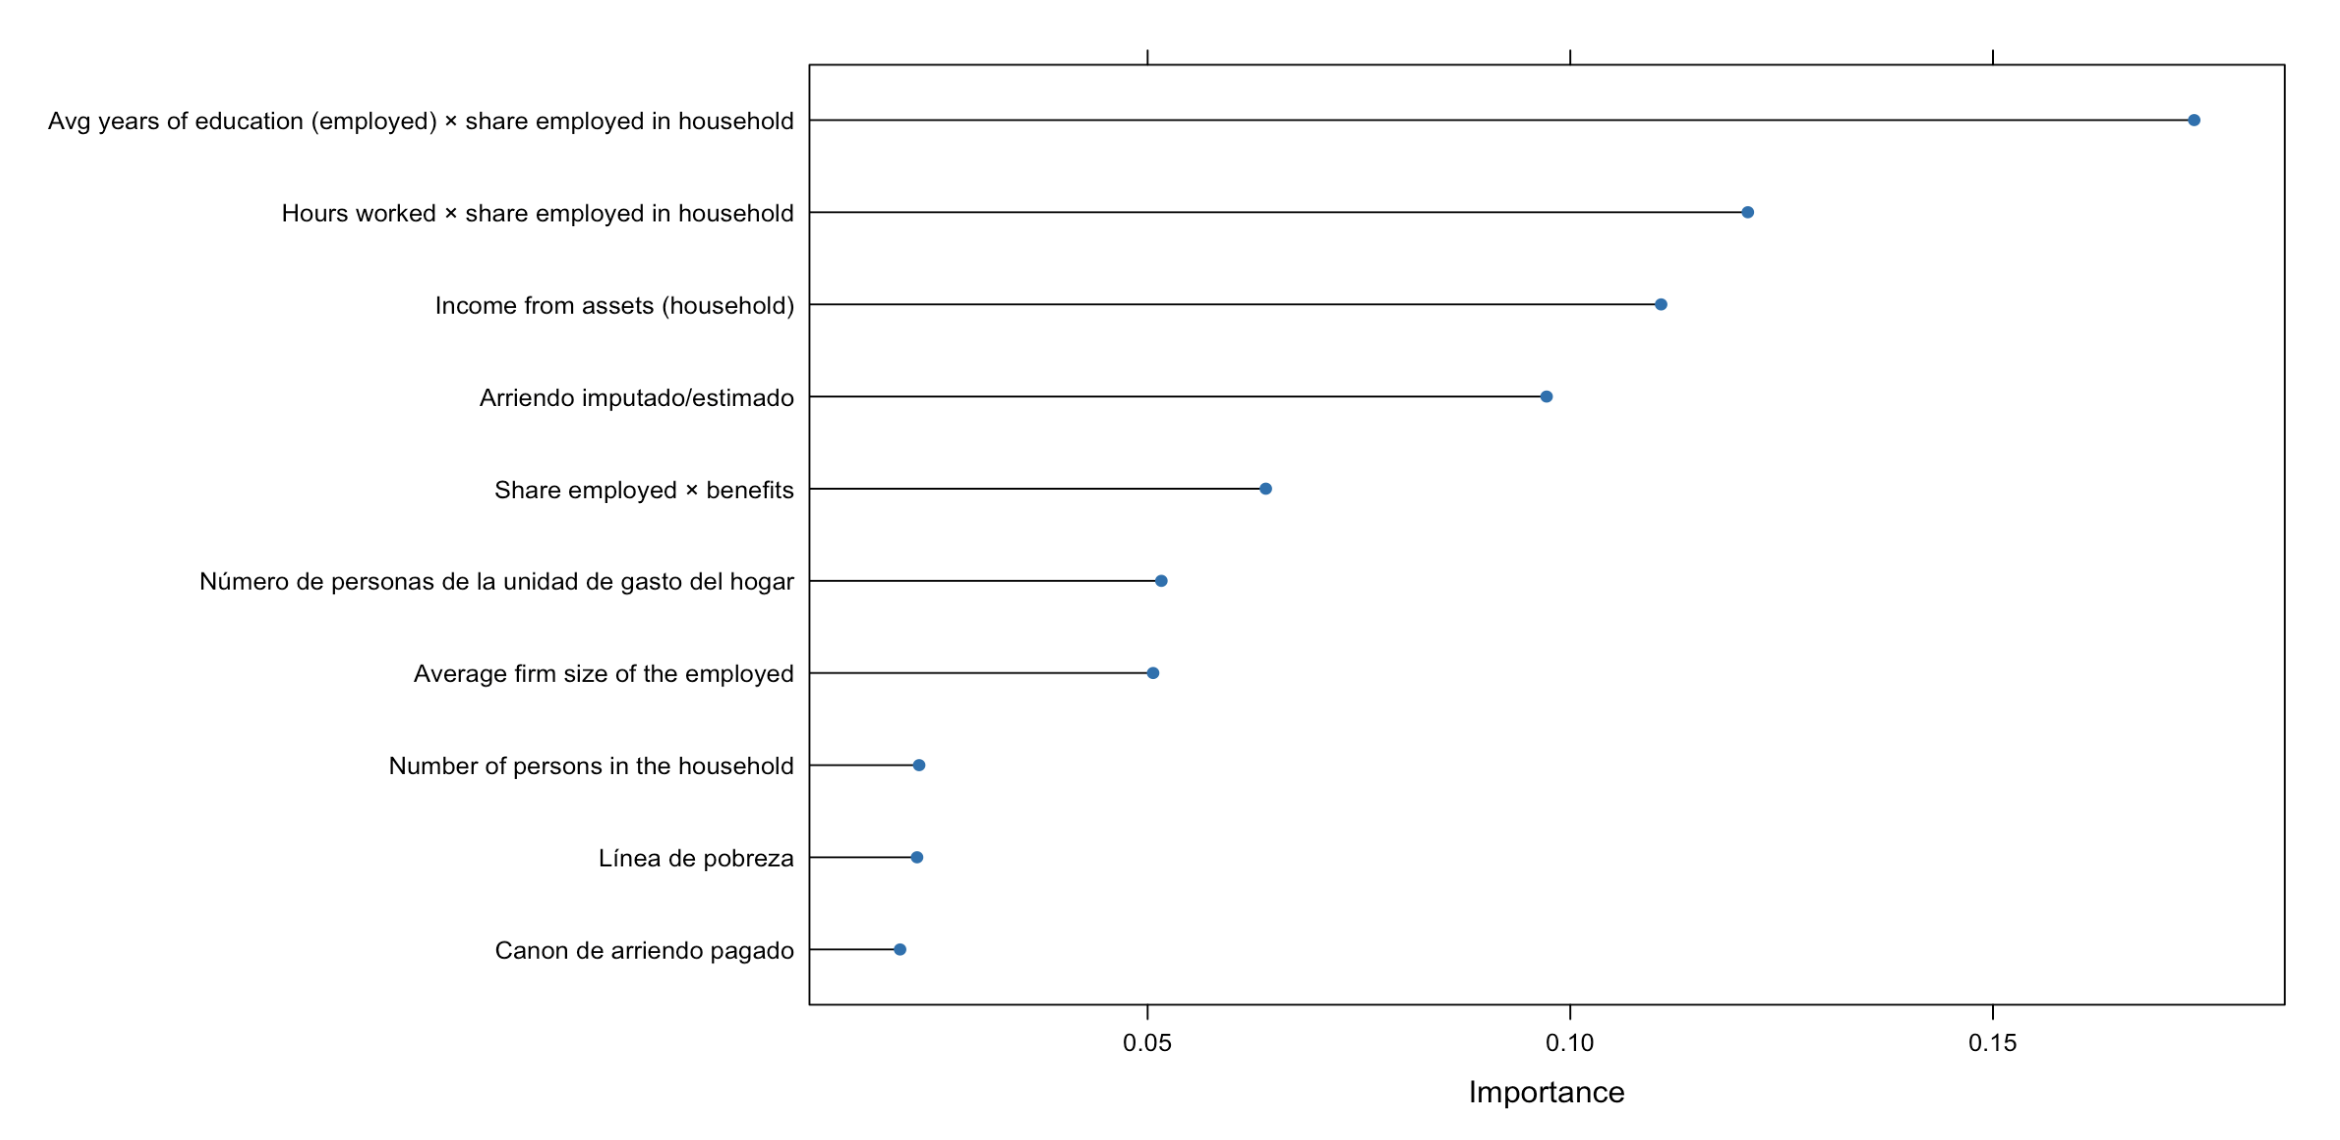
\includegraphics[width=1\linewidth]{importance xgboost.png}
    \caption{Top 10 Relative Importance of Variables in XGBoost}
    \label{fig:placeholder}
\end{figure}


 \begin{table}[h!]
 \footnotesize
\caption{Trained Models - Results Metrics} 
\centering
\begin{tabular}{l c c c c c c c}
\hline
\textbf{Model} & \textbf{Precision} & \textbf{Recall} & \textbf{In-sample F1} & \textbf{Out-of-sample F1}  \\
\hline
Logit 1 & 0.65 & 0.24 & 0.35  &    0.36   \\
Logit 2 & 0.70 &  0.46 & 0.55 &    0.57   \\
Logit 3 & 0.71 & 0.53  &  0.61 & 0.62   \\
Elastic Net  1    & 0.57 & 0.73  & 0.65  & 0.65\\
CART 1   & 0.66 & 0.47  & 0.55 & 0.48      \\
Random Forest 1    & 0.90 & 0.75  & 0.82 &  0.65      \\
Random Forest 2 & 0.79 & 0.91  & 0.84  & 0.68    \\
Random Forest 3  & 0.77 & 0.92  & 0.85  & 0.69   \\
Gradient Boosting 1    & 0.64 & 0.77  &  0.70 &  0.70   \\
Random Forest 4  & 0.80 & 0.92  & 0.86  &  0.71    \\
Random Forest 5 & 0.75 &  0.87 & 0.80  &  0.70     \\
Gradient Boosting 2    &0.68 & 0.79  & 0.72  &   0.72  \\
\textbf{Extreme Gradient Boosting 1} & 0.71 & 0.78  & 0.74  &  \textbf{0.74}    \\
\textbf{Extreme Gradient Boosting 2}    &0.70 & 0.79  & 0.74  &   \textbf{0.74}  \\

\hline
\end{tabular}
\vspace{0.5em}
\small{\parbox{\linewidth}{%

}}
\end{table}


Finally, the preceding results are summarized in Table 3. As shown, each step in the process was designed to test different optimization strategies—whether in feature engineering, methodology selection, or hyperparameter tuning—and to assess whether their inclusion enhanced or hindered the model’s ability to predict “pobre.” All insights obtained during these initial experiments were incorporated into our final model, \textbf{Extreme Gradient Boosting 2}, which consolidated every progressive improvement achieved throughout this experimental process.

Reaching this outcome—and understanding why this final model outperformed the others, even achieving the highest F1 score in the Kaggle competition with less than half the submission attempts of the next best team—reflects the central principle that guided this study: Our modeling strategy followed an experimental and incremental approach varying one component at a time and measured its impact on out-of-sample performance. 

\section{Conclusion}

This project set out to answer a simple but powerful question: \textit{Can we accurately predict poverty in Colombia using fewer, cheaper, and more accessible variables?} Addressing this question was not only a computational challenge but also a conceptual one, requiring us to carefully define the problem, understand the data, and test multiple solutions through rigorous experimentation.

Throughout the process, we trained a wide range of models--from simple logistic regressions to regularized and aggregation methods--each evaluated with the same objective metric: out-of-sample F1 score. Among these, three stood out for their performance: Random Forest (F1 = 0.71), Gradient Boosting (F1 = 0.72), and ultimately, Extreme Gradient Boosting (XGBoost), which reached the highest out-of-sample F1 score of 0.74. 

Why did XGBoost outperform all others? We believe it is the result of three converging factors. First, the model’s ability to capture low-order interactions through shallow trees aligned perfectly with our carefully crafted feature set. Second, extensive hyperparameter tuning helped regularize the model and minimize overfitting, while threshold optimization aligned the classifier with the F1 metric under class imbalance. Finally, our use of out-of-fold predictions to calibrate the decision threshold provided a more stable and accurate evaluation of performance, especially in the presence of skewed classes.

The variables included in this final model reflect meaningful economic signals of poverty: household labor intensity, human capital, and demographic structure. Variables such as the proportion of employed members, average hours worked, and educational attainment--not just of the household head, but of all working members--proved to be key predictors. These results not only validate our domain-driven feature engineering process, but also highlight the possibility of predicting poverty with structural and observable indicators, rather than relying on hard-to-measure income data.

Looking ahead, a promising path to further improve these results is to train a Light Gradient Boosting Machine (LightGBM) model, whose preliminary in-sample tests showed potential for higher performance. Additionally, future work could explore the use of transfer learning or ensemble methods, which combine multiple base models into a meta-learner to reduce overfitting and enhance generalization. Finally, narrowing down the model to a parsimonious set of highly informative features--without compromising performance--remains a valuable goal for practical deployment in policy settings.

In retrospect, this work illustrates that learning in machine learning should not be reduced to optimization. As \href{https://x.com/lateinteraction/status/1979612318255456353}{recent discussions} in the field suggest, genuine learning involves reflection and understanding—qualities that enable efficient exploration beyond gradient-based search. Our approach sought precisely that: to narrow the decision space through a deep understanding of the problem and domain knowledge before brute-force experimentation. While in practice, the process itself was far more exploratory and improvisational than the structured account presented here, this reconstruction captures the essence of learning as we understand it: the emergence of order and insight from a process that was, at its core, iterative and uncertain.

\clearpage


\bibliography{References}

%apaendice 1
\section{Appendix}
\renewcommand{\thetable}{A\arabic{table}}
\setcounter{table}{0}

\subsection{Variable Set}

Table A1 reports the feature set used in our models: 10 original household fields kept as-is; 41 engineered household-level aggregates built from 36 distinct person-module questions; and 9 higher-order terms (7 interactions, 2 squares) that add no new questions. None of the 10 household fields are double-counted in the 36. In total, the design draws on 46 unique survey items. 

\begin{longtable}{p{4cm} p{2.4cm} p{9.6cm}}
\caption{Feature Set: Original Variables, Household Aggregates, and Interactions}\\
\label{tab:A1}
\toprule
\textbf{Variable} & \textbf{Type} & \textbf{Definition / Construction}\\
\midrule
\endfirsthead
\toprule
\textbf{Variable} & \textbf{Type} & \textbf{Definition / Construction}\\
\midrule
\endhead
\midrule
\multicolumn{3}{r}{\emph{Continues on next page}}\\
\bottomrule
\endfoot
\bottomrule
\endlastfoot

\multicolumn{3}{l}{\textbf{Panel 1. Original variables included in the model}}\\
\addlinespace
\texttt{P5000} & Numeric & Total rooms in the dwelling (includes living-dining; excludes kitchen/bath/garage if only a vehicle is stored).\\
\texttt{P5010} & Numeric & Rooms used for sleeping.\\
\texttt{P5090} & Categorical & Tenure status (owned paid, owned paying, rent, usufruct, possession without title, other).\\
\texttt{P5100} & Numeric & Monthly mortgage or loan payment for the dwelling (if applicable).\\
\texttt{P5130} & Numeric & Imputed monthly rent (owners, usufruct, occupants de facto).\\
\texttt{P5140} & Numeric & Monthly rent paid (excludes building fee or concierge).\\
\texttt{Nper} & Integer & Number of persons in the household.\\
\texttt{Npersug} & Integer & Number of persons in the expenditure unit.\\
\texttt{Depto} & Categorical & Department code.\\
\texttt{Lp} & Numeric & Official monetary poverty line.\\

\addlinespace
\multicolumn{3}{l}{\textbf{Panel 2. Aggregates from individuals to household level}}\\
\addlinespace

\multicolumn{3}{l}{\emph{Counts and labor force status}}\\
\texttt{n\_personas} & Integer & Household size: number of individuals in the household.\\
\texttt{n\_occ} & Integer & Employed persons: sum of 1\{Oc = 1\}.\\
\texttt{n\_des} & Integer & Unemployed persons: sum of 1\{Des = 1\}.\\
\texttt{n\_ina} & Integer & Inactive persons: sum of 1\{Ina = 1\}.\\
\texttt{n\_pet} & Integer & Labor force (original PET): sum of 1\{Pet = 1\}.\\
\texttt{n\_pet\_flex} & Integer & Labor force (flexible definition): sum of 1\{PET\_flexible = 1\}.\\
\texttt{n\_no\_pet\_flex} & Integer & Non-labor force (flexible): n\_personas minus n\_pet\_flex.\\
\texttt{n\_occ\_in\_pet\_flex} & Integer & Employed within flexible PET: sum of 1\{Oc = 1 and PET\_flexible = 1\}.\\

\multicolumn{3}{l}{\emph{Composition ratios}}\\
\texttt{prop\_occ\_nper} & Numeric & n\_occ divided by n\_personas (safe division, returns 0 if denominator $\le$ 0).\\
\texttt{prop\_des\_nper} & Numeric & n\_des divided by n\_personas (safe division).\\
\texttt{prop\_ina\_nper} & Numeric & n\_ina divided by n\_personas (safe division).\\
\texttt{prop\_no\_pet\_nper} & Numeric & n\_no\_pet\_flex divided by n\_personas (flexible PET).\\
\texttt{prop\_occ\_pet} & Numeric & n\_occ divided by n\_pet (employment rate in original PET).\\
\texttt{prop\_occ\_pet\_flex} & Numeric & n\_occ\_in\_pet\_flex divided by n\_pet\_flex (flexible PET).\\

\multicolumn{3}{l}{\emph{Household head (P6050 = 1)}}\\
\texttt{edad\_jefe} & Numeric (years) & Age of head: first P6040 where P6050 = 1.\\
\texttt{sexo\_jefe} & Categorical & Sex of head: first P6020 where P6050 = 1.\\
\texttt{tam\_emp\_jefe} & Numeric & Firm size of head: first P6870 at P6050 = 1 (NA to 0).\\
\texttt{cotiza\_pens\_jefe} & Binary \{0,1\} & Pension contribution: first P6920 at P6050 = 1 (coalesced).\\
\texttt{pos\_ocup\_jefe} & Categorical & Occupational position: first P6430 at P6050 = 1 (coalesced).\\
\texttt{antig\_jefe} & Numeric (months) & Job tenure: first P6426 at P6050 = 1 (NA to 0).\\
\texttt{jefe\_max\_edu} & Ordinal code & Maximum education code among head records: max P6210 at P6050 = 1 (NA removed).\\
\texttt{jefe\_max\_edu\_years} & Numeric & Same as above but forced finite (non-finite to 0).\\
\texttt{jefe\_ocupado} & Binary \{0,1\} & Indicator that head is employed: exists\{P6050 = 1 and Oc = 1\}.\\
\texttt{prestaciones\_jefe} & Binary \{0,1\} & Any benefit for head in \{P6510, P6545, P6580, P6630s1, s2, s3, s4, s6\}.\\
\texttt{horas\_jefe} & Numeric & Weekly hours for head if employed: first P6800 at P6050 = 1 and Oc = 1; otherwise 0.\\

\multicolumn{3}{l}{\emph{Job quality (household level)}}\\
\texttt{prestaciones} & Binary \{0,1\} & Any household member with benefits in \{P6510, P6545, P6580, P6630s1, s2, s3, s4, s6\}.\\
\texttt{prop\_prest\_occ} & Numeric [0,1] & Among employed (Oc = 1): share with any benefit; 0 if n\_occ = 0.\\

\multicolumn{3}{l}{\emph{Averages among employed (Oc = 1)}}\\
\texttt{prom\_horas\_occ} & Numeric & Mean P6800 given Oc = 1; 0 if none employed.\\
\texttt{tam\_emp\_prom\_occ} & Numeric & Mean P6870 given Oc = 1; 0 if none employed.\\
\texttt{antig\_prom\_occ} & Numeric & Mean P6426 given Oc = 1; 0 if none employed.\\
\texttt{mean\_edu\_occ} & Numeric (years) & Mean edu\_years given Oc = 1; 0 if none employed.\\
\texttt{edad\_prom\_occ} & Numeric (years) & Mean P6040 given Oc = 1; 0 if none employed.\\

\multicolumn{3}{l}{\emph{Second job}}\\
\texttt{segundo\_trabajo\_hogar} & Binary \{0,1\} & Any member reports a second job: exists P7040 = 1.\\
\texttt{horas\_segundo\_trabajo\_prom} & Numeric & Mean P7045 given P7040 = 1; 0 if none.\\

\multicolumn{3}{l}{\emph{Unemployment with income (household classification)}}\\
\texttt{n\_desoc\_con\_ingresos} & Integer & Sum of 1\{Des = 1 and (P7422 = 1 or P7472 = 1)\}.\\
\texttt{desoc\_con\_ingresos\_cat} & Factor (3 levels) & Based on n\_des and n\_desoc\_con\_ingresos: sin\_desocupados (no unemployed), desoc\_con\_ingresos (unemployed with income), desoc\_sin\_ingresos (unemployed without income).\\

\multicolumn{3}{l}{\emph{Child labor and seniors}}\\
\texttt{child\_work\_cat} & Factor (3 levels) & Among ages 10 to 14 with Oc = 1 and schooling P6240: none, work\_study (P6240 = 3), work\_no\_study (P6240 not 3).\\
\texttt{senior\_work\_cat} & Factor (3 levels) & Seniors 65+ working by education: none, calificado (edu\_years $\ge$ 16), no\_calificado (edu\_years $<$ 16).\\

\multicolumn{3}{l}{\emph{Non-labor income indicators}}\\
\texttt{ingreso\_por\_activos} & Binary \{0,1\} & Any of \{P7495 = 1, P7500s2 = 1, P7510s5 = 1\}.\\
\texttt{ingreso\_otros} & Binary \{0,1\} & Any of \{P7505 = 1, P7510s7 = 1\}.\\
\texttt{ingreso\_ayudas} & Binary \{0,1\} & Any of \{P7510s1 = 1, P7510s2 = 1, P7510s3 = 1\} or P7500s3 = 1 or P7510s7 = 1.\\

\addlinespace
\multicolumn{3}{l}{\textbf{Panel 3. Nonlinear terms and interactions}}\\
\addlinespace
\texttt{edad\_jefe2} & Numeric & Square of head age: (edad\_jefe)$^2$.\\
\texttt{edad\_prom\_occ2} & Numeric & Square of mean age among employed: (edad\_prom\_occ)$^2$.\\
\texttt{sexo\_desocup} & Numeric & sexo\_jefe times prop\_des\_nper.\\
\texttt{edu\_occ\_lp} & Numeric & mean\_edu\_occ times Lp.\\
\texttt{horasxedu\_occ} & Numeric & prom\_horas\_occ times mean\_edu\_occ.\\
\texttt{horasxpropocc} & Numeric & prom\_horas\_occ times prop\_occ\_nper.\\
\texttt{meanedu\_x\_propocc} & Numeric & mean\_edu\_occ times prop\_occ\_nper.\\
\texttt{propocc\_x\_lp} & Numeric & prop\_occ\_nper times Lp.\\
\texttt{propocc\_x\_prest} & Numeric & prop\_occ\_nper times prop\_prest\_occ.\\

\end{longtable}


\end{document}

